% !TEX TS-program = pdflatex   
\documentclass[runningheads,12pt]{article} 
\usepackage{textcomp,color,longtable,landscape,float}
\restylefloat{table}
\def\headerTitle{CSE4312F12 Project -- ROI Solution}
\usepackage{sty/bsymb} %% Event-B symbols
\usepackage{sty/eventB} %% REQ and ENV
%%UML
%UML
\usepackage{tikz}
%\usepackage[school,simplified]{pgf-umlcd}
%\usepackage[simplified]{sty/pgf-umlcd}
\usepackage{mdframed}%% put frame around a table
\usepackage{rotating} 
\usepackage{subfigure}
\usepackage{sty/CalcStyleV8}

\def\newlineindent{\newline\indent}
\def\require{\quad\textbf{require}~}           
\def\ensure{\quad\textbf{ensure}~}
\def\param{\quad\textbf{param}~}
\def\where{\quad\textbf{where}~}
\def\when{\quad\textbf{when}~}
\def\axiom{\textbf{axiom}~}
\def\comment{\quad \texttt{--}}
\def\ddo{\quad\textbf{do}~} 
\def\any{\quad\textbf{any}~}   
\def\cset{\textbf{carrier set}~}
\def\var{\textbf{var}~}
\def\const{\textbf{const}~}
\def\is{~\textbf{is}~}
\def\suchthat{\,|\,}
\def\yields{\,\bullet\,}
\def\itholds{\,\bullet\,}
\def\inv{\textbf{inv}~}
\def\eqdef{~\triangleq~}
\def\event{\textbf{event}~}
\def\proc{\textbf{proc}~}
\def\query{\textbf{query}~}
\def\init{\textbf{init}~}
\def\use{\textbf{use}~}
\def\constraint{\textbf{constraint}~}
\def\property{\textbf{property}~}
\def\regexp{REGEXP}
\def\infix{\textbf{infix }}
\def\prefix{\textbf{prefix }}
\def\dummy{\textbf{dummy }}
\def\theorem{\textbf{theorem }}
\def\squote#1{\textrm{\textquotesingle#1\textquotesingle}}

\usepackage{listings,xcolor}%%lstlang0.sty
\definecolor{codebg}{rgb}{0.92,0.92,0.92}      

\usepackage{multirow}    
\usepackage{pbox}

% block in math mode
\def\block{\array{@{}l@{}}}
\let\endblock=\endarray

% Inline Eiffel Code
\newcommand{\e}[1]{\lstinline[language=OOSC2Eiffel]|#1|}


% Eiffel figure setup
\lstnewenvironment
  {ecodel}[1][]
  {\lstset{language=OOSC2Eiffel,float=htb,columns=fullflexible,backgroundcolor=\color{codebg},captionpos=b,
  xleftmargin=1cm,numberfirstline=true,numberstyle=\hspace*{1cm},numbers=left,mathescape=true,#1}}
  {}

\lstnewenvironment
  {ecodel2}[1][]
  {\lstset{language=OOSC2Eiffel,float=htb,columns=fullflexible,backgroundcolor=\color{codebg},captionpos=t,
  xleftmargin=1cm,mathescape=true,#1}}
  {}
                          
%%%%% Pretty print an Eiffel feature
%%%%% Arguments:
%%%%% 1. Name of the routine, parameters and return type if applicable.
%%%%% 2. Comments of the routine.
%%%%% 3. Pre-condition (can be split into multiple lines; math symbols must be enclosed within $...$)
%%%%% 4. Implemnetation (it's recommanded that use \texttt{...} to wrap each line to emphasize that it's code, not spec.)
%%%%% 5. Post-condition (can be split into multiple lines; math symbols must be enclosed within $...$)
%%%%%
%%%%% Usage: \feature{f (params) : return }{comment}{pre}{do}{post}  
%%%%%       will produce the following
%%%%%
%%%%%       f (params) : return
%%%%%       		-- comment
%%%%%       	require pre
%%%%%          	do
%%%%%				imp
%%%%%			ensure post
%%%%%			end        
%%%%% Special case:
%%%%% - Contract view --> \feature{f (params) : return }{comment}{pre}{}{post} 
%%%%% - Precondition only -->  \feature{f (params) : return }{comment}{pre}{}{} 
%%%%% - Postcondition only --> \feature{f (params) : return }{comment}{}{}{post}      
%%%%% - Implementation only --> \feature{f (params) : return }{comment}{}{imp}{} 

\def\requires{\textbf{require}}           
\def\ensures{\textbf{ensure}}    
\def\Do{\textbf{do}}
\def\End{\textbf{end}}   
                                        
\newlength{\requirewidth}
\settowidth{\requirewidth}{require}  
\def\old{\mathop{\textbf{old}}}   

\newcommand\contract[2]{  
	\begin{array}{@{\quad}l@{\quad}l}
	\begin{minipage}[t]{\widthofpbox{#1}} #1 \end{minipage} 
	&
	\begin{minipage}[t]{\widthofpbox{#2}} #2 \end{minipage}
	\end{array}}             

\newcommand{\feature}[5]{
  \def\comments{#2}
  \def\pre{#3}
  \def\imp{#4}
  \def\post{#5}     
  \begin{array}[!htbp]{|@{\quad}l@{\quad}|}
    \hline
    \\[-1ex]
    #1 \\   

	\ifx\comments\empty
	\else
	\quad\quad\text{-}\text{- }\text{\comments} \\
	\fi   
	
	\ifx\pre\empty
	\else                        
		\contract{\requires}{\pre} \\
	\fi  
	
	\ifx\imp\empty
	\else
	\begin{array}[!htbp]{@{\quad}l}
	    \Do \\ 
	    \begin{array}[!htbp]{@{\quad}l}
			\imp
		\end{array}
	\end{array}\\
	\fi        
	
	\ifx\post\empty
	\else
	\contract{\ensures}{\post} \\
	\fi 
	  
	\ifx\imp\empty 
	% contract view
    \else
     \quad\Bend
    \fi \\[1ex] 
    \hline
  \end{array}
}

\newcommand{\module}
{
 \begin{array}[!htbp]{|@{\quad}l@{\quad}|}
    \hline
   
    \hline
  \end{array}
}

\usepackage{amssymb,amsmath}
\setcounter{tocdepth}{3}
\usepackage{graphicx}
%\usepackage[text={16cm,23cm}]{geometry} %% use more of the page
\usepackage{url} 

\usepackage{enumitem} 
\usepackage{float,afterpage}
\usepackage{caption}

%reduce spacing in lists
\usepackage[section]{placeins}
\setlist{nolistsep,leftmargin=*} 

\usepackage{fancyhdr,lastpage}
\lhead{\rm \headerTitle}
\rhead {\rm Page \thepage~of \pageref{LastPage}}
\lfoot{}\cfoot{}\rfoot{}
\pagestyle{fancy}

%%%%%%%%%Definitions%%%%%%%%%%

\def\implies{\Rightarrow } 
\def\Fl{\mathbb{F}}%%FLOAT
\def\Bl{\mathbb{B}}%%BOOLEAN
\def\St{\mathbb{S}}%%STRING
%%%%%%%%%%%%%%%%%%%%%%%%%%%%

%For reducing size of section headings
\usepackage{sectsty}
\sectionfont{\normalsize}
\subsectionfont{\small}
\subsubsectionfont{\small}
\usepackage{titlesec}
\titlespacing*{\section}{0pt}{*1.2}{*0.5}
\titlespacing*{\subsection}{0pt}{*0.5}{*0.5}
\titlespacing*{\subsubsection}{0pt}{*0.5}{*0.5}

%http://www.eng.cam.ac.uk/help/tpl/textprocessing/squeeze.html
%By default, LaTeX doesn't like to fill more than 0.7 of a text page with tables and graphics, nor does it like too many figures per page. This behaviour can be changed by placing lines like the following before \begin{document}
\renewcommand\floatpagefraction{.9}
\renewcommand\topfraction{.9}
\renewcommand\bottomfraction{.9}
\renewcommand\textfraction{.1}   
\setcounter{totalnumber}{50}
\setcounter{topnumber}{50}
\setcounter{bottomnumber}{50}

%\usepackage{CalcStyleV8}
%\usepackage{subfigure}


\usepackage{sty/tikz-uml}%% Put this last
\usepackage{lscape}
 
\hyphenpenalty 10000


\begin{document}

\title{CSE4312F12 Project Solution\\
ROI}

\author{Damien Gruel (cse23089@cse.yorku.ca)
\and Ludovic Lavalette (cse23088@cse.yorku.ca)}

\date{\today}

\maketitle


\section*{Note}
\begin{itemize}
\item A customer elicitation session was held during class on Tuesday November 6, 2012. If you were not there sure to catch up with a fellow student who was there.
\item This template is handed out \emph{caveat emptor}.  There may be errors and wrong information. It is ultimately your responsibility to elicit the correct requirements from the customer and to ensure that you satisfy the customer goals and specify correct output from the input.
\item Your are required to correct any errors or ambiguities in this template and use this template to produce your final requirements document.
\end{itemize}

\section*{Revisions}

\begin{tabular}{|l|l|p{3in}|}
\hline
Date & Revision& Description \\ 
\hline
10 October  2012 
& 1.0       
& Initial customer elicitation\\ 
\hline
15 November 2012
& 2.0       
& Initial Student solution       \\
\hline
1 December 2012
& 3.0       
& Final Student solution       \\
\hline
\end{tabular}

\newpage
\tableofcontents
\listoffigures
\listoftables

\newpage

\section{Context Diagram}



The following diagram is the context diagram for the ROI system.\\
\\
The monitored variables (which are the content of the CSV file, provided by the user), are :
\begin{itemize}
\item an header, which is composed of a required name, an optional description of the file and optional information about the customer (account number, email, address and phone number)
\item the evaluation dates (\textit{start} and \textit{end})
\item the tuple data (\textit{date}, \textit{market value}, \textit{cash flow}, \textit{agent fees} and \textit{benchmark}).
\end{itemize}
\bigskip
The format of the output is the following (whole input = everything between the earliest date and the latest date in the sequence of tuple data):\\
\\
Name: ??\\
--------------------------------------------\\
Whole input: yyyy-mm-dd to yyyy-mm-dd\\
TWR: ?? \%\\
ROI: ?? \%\\
Benchmark: ?? \%\\
--------------------------------------------\\
Evaluation Period: yyyy-mm-dd to yyyy-mm-dd\\
TWR: ?? \%\\
ROI: ?? \%\\
Benchmark: ?? \%\\
--------------------------------------------\\
\\
\\
The controlled variables are also a warning (if a calculation is not possible, if the evaluation period is not valid, or if the portfolio history has no name) and an error (if the CSV file is not valid).\\

\begin{figure}
\centering
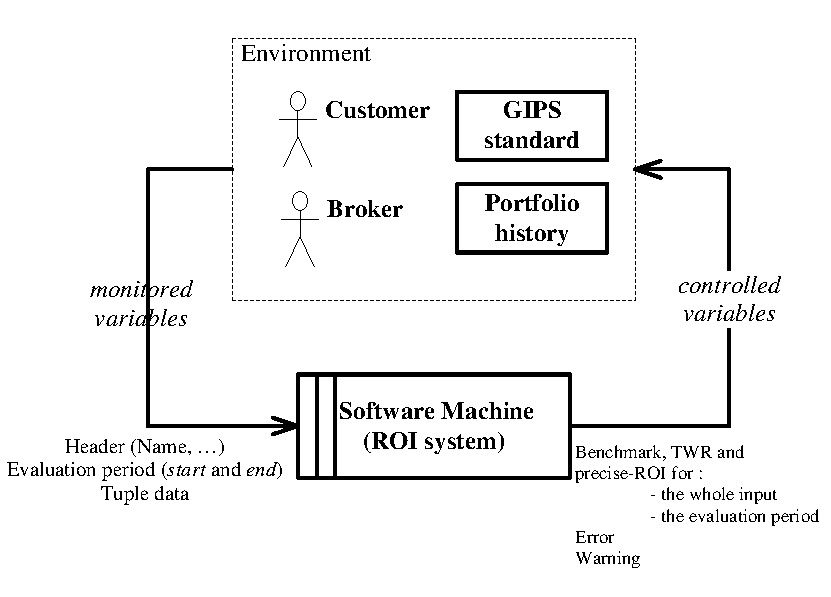
\includegraphics[scale=1.0]{inputs/context.pdf}
\caption{Context diagram for the ROI system}
\label{fig:ROI-context}
\end{figure}
\section{Dictionary}

\smallskip


\noindent\textbf{Agent fees}: Money that the customer pays to the investment advisor to run the account.\smallskip

\noindent\textbf{Benchmark}: Standard used as a point of reference for evaluating performance.\smallskip

\noindent\textbf{Cash Flow}: Revenue or expense stream that changes a cash account over a given period.\smallskip

\noindent\textbf{CSV}: Comma Separated Value file format used to store tabular data in which numbers and text are stored in plain-text form that can be easily written and read in a text editor.\smallskip

\noindent\textbf{Customer}: The user of the software system.\smallskip

\noindent\textbf{Evaluation Period}: a start and end date (provided by the user) for the portfolio history over which the return on investment is calculated.\smallskip

\noindent\textbf{GIPS}: Global Investment Performance Standards\smallskip

\noindent\textbf{Investment broker}: Runs the portfolio on behalf of the customer and supplies portfolio accounts.\smallskip

\noindent\textbf{Portfolio statement}: List of all investments and current value.\smallskip

\noindent\textbf{Portfolio History}: the historical data of investment performance over time that the customer stores about their investments as gleaned from their monthly or yearly investment accounts. Usually stored by customers in a CSV file (see Figure 1).\smallskip

\noindent\textbf{ROI}: Return On Investment: Performance measure used to evaluate the efficiency of an investment.\smallskip

\noindent\textbf{TWR}: Time Weighted Return: Measure of the compound rate of growth in a portfolio.\smallskip

\noindent\textbf{Tuple data}: \textit{date}, \textit{market value}, \textit{cash flow}, \textit{agent fees} and \textit{benchmark}.\smallskip

%%%%%%%%%%%%%%%%%%%%%%%%%%%%%%%%%%%
\section{E/R-descriptions}

\subsection{E-descriptions}

{\centering
\begin{longtable}{|l|p{9cm}|p{5cm}|}
\hline
\textbf{ID} & \textbf{Description} & \textbf{Comment}\\

\hline
E1 & Customers create and store a portfolio history, i.e. the historical data of their investment performance as determined from portfolio statements. & \\

\hline
E2 & Customers store their portfolio history as a CSV text file. CSV files may be prepared on editors of any operating system and encoded as ANSI or UTF-8. & \\

\hline
\end{longtable}
%%%


%%%
\centering
\begin{longtable}{|l|p{9cm}|p{5cm}|}

\hline
\multicolumn{3}{|c|}{\textbf{Header of the CSV file}} \\


\hline
E3.1 & Every portfolio history has a name. & \\

\hline
E3.2 & Optionally, every portfolio history has a description, account number, email, address, and phone number fields. & \\

\hline
\end{longtable}
%%%

%%%
\centering
\begin{longtable}{|l|p{9cm}|p{5cm}|}

\hline
\multicolumn{3}{|c|}{\textbf{Evaluation period in the CSV file}} \\

\hline
E4.1 & Optionally, every portfolio has an evaluation period that is between the start and end date of the historical performance data. & See Invariant 1 of TWR\_ROI\_CALCULATION (Fig.~\ref{tab:twr_calculation})\\

\hline
E4.2 & The start date and the end date must be in ISO format (yyyy-mm-dd). & \\

\hline
E4.3 & The evaluation period is in range. & See Invariant 1 of TWR\_ROI\_CALCULATION (Fig.~\ref{tab:twr_calculation})\\

\hline
\end{longtable}
%%%

%%%
\centering
\begin{longtable}{|l|p{9cm}|p{5cm}|}

\hline
\multicolumn{3}{|c|}{\textbf{Data in the CSV file}} \\

\hline
E5.1 & A portfolio history records investment performance in a non-empty sequence of tuple data, each tuple having the fields: date (required), market value (required), cash flow (optional), agent fees (optional) and benchmark (optional). & See \textit{tr} of TWR\_ROI\_CALCULATION (Fig.~\ref{tab:twr_calculation})\\

\hline
E5.2 &  For each tuple, the dates must be in ISO format (yyyy-mm-dd). & \\

\hline
E5.3 & When there is a customer contribution, the cash flow is a positive number. For a withdrawal, the number is negative. & \\

\hline
E5.4 & Agent fees can be internal (deducted from within the portfolio) or external (additional amounts paid by the customer to the investment broker). The portfolio history reflects only external agent fees, always reported as a non-negative amount. & \\

\hline
E5.5 & Every data tuple (row in the CSV file) has a date and a non-negative market value. & See Invariant 2 of TWR\_ROI\_CALCULATION (Fig.~\ref{tab:twr_calculation})\\

\hline
E5.6 &  Dates in the tuples are unique and ordered. & See Invariant 3 of TWR\_ROI\_CALCULATION (Fig.~\ref{tab:twr_calculation})\\

\hline
E5.7 & No withdrawal in the tuple data can be greater than the market value. & See Invariant 4 of TWR\_ROI\_CALCULATION (Fig.~\ref{tab:twr_calculation})\\

\hline
E5.8 & An account cannot grow from zero market value and cash flow. & See Invariant 5 of TWR\_ROI\_CALCULATION (Fig.~\ref{tab:twr_calculation})\\

\hline
E5.9 &  For each tuple, the market value plus cash-flow plus agent-fees must be non-zero. & See precondition 3 of feature \textit{twr} of TWR\_ROI\_CALCULATION (Fig.~\ref{tab:twr_calculation})\\

\hline
\end{longtable}
}


%%%%%%%%%%%%%%%%
\subsection{R-descriptions}

{\centering
\begin{longtable}{|l|p{9cm}|p{5cm}|}
\hline
\textbf{ID} & \textbf{Description} & \textbf{Comment}\\

\hline
R1 & All return on investment calculations shall follow the GIPS standard. & See twr, roi, benchmark (Fig.~\ref{tab:twr_calculation}) \\

\hline
\end{longtable}
%%%
\centering
\begin{longtable}{|l|p{9cm}|p{5cm}|}
\hline
\multicolumn{3}{|c|}{\textbf{Evaluation period}} \\

\hline
R2.1 & If no evaluation period is provided, then the start date is the earliest date and the end date the latest date in the sequence of tuple data. & See Start\_Valid and End\_Valid conditions of the function tables\\

\hline
R2.2 &  Warning message: If the evaluation dates are not valid, then the following error message shall be displayed to the user: "Invalid evaluation period" & See Function tables \\

\hline
\end{longtable}
%%%
\centering
\begin{longtable}{|l|p{9cm}|p{5cm}|}

\hline
\multicolumn{3}{|c|}{\textbf{CSV file}} \\

\hline
R3.1 &  Error message: If the CSV file is not valid (i.e. if any of the conditions mentioned above do not hold), then the following error message shall be displayed to the user: "Invalid file". & See Function tables\\

\hline
R3.2 &  Warning message: If the CSV file does not contain a name, then the following error message shall be displayed to the user: "Incomplete file: absence of name". & See Function table~\ref{table:ftable_name}\\

\hline
\end{longtable}
%%%
\centering
\begin{longtable}{|l|p{9cm}|p{5cm}|}

\hline
\multicolumn{3}{|c|}{\textbf{Calculation of the TWR}} \\

\hline
R4.1 & The system shall provide two TWRs (if each one is calculable) : one for the evaluation period, and one for the whole input. & See Function table~\ref{table:ftable_TWR} \\

\hline
R4.2 &  The TWRs shall be rounded to two decimal places. & \\

\hline
R4.3 & If the evaluation period is less than a year, then the TWR shall be reported in absolute terms as a percentage return (i.e. it is not annualized). If the evaluation period is a year or more, then the TWR is annualized to a percentage per year. & See postcondition of  \textit{annual\_compounded\_TWR} of TWR\_ROI\_CALCULATION (Fig.~\ref{tab:twr_calculation})\\

\hline
R4.4 & The annualized TWR shall be reported as a percentage. & See \textit{annual\_compounded\_TWR} of TWR\_ROI\_CALCULATION (Fig.~\ref{tab:twr_calculation})\\

\hline
R4.5 & Agent fees are treated like a deposit (the agent fees are \underline{added} to the market value and the cash flow). & See \textit{twr} of TWR\_ROI\_CALCULATION (Fig.~\ref{tab:twr_calculation})\\

\hline
R4.6 & Warning message: If the TWR is not calculable, then a warning message shall be displayed to the user. & See Function table~\ref{table:ftable_TWR}\\

\hline
\end{longtable}
%%%
\centering
\begin{longtable}{|l|p{9cm}|p{5cm}|}

\hline
\multicolumn{3}{|c|}{\textbf{Calculation of the ROI}} \\

\hline
R5.1 & The system shall provide two ROIs : one for the evaluation period, and one for the whole input. & See Function table~\ref{table:ftable_ROI}\\

\hline
R5.2 &  The ROIs shall be rounded to two decimal places. & \\

\hline
R5.3 & The ROI shall be reported as a percentage. & See \textit{roi} of TWR\_ROI\_CALCULATION (Fig.~\ref{tab:twr_calculation})\\

\hline
R5.4 & Agent fees are treated like a deposit (the agent fees are \underline{added} to the cash flow). & See \textit{roi} of TWR\_ROI\_CALCULATION (Fig.~\ref{tab:twr_calculation})\\

\hline
\end{longtable}
%%%
\centering
\begin{longtable}{|l|p{9cm}|p{5cm}|}

\hline
\multicolumn{3}{|c|}{\textbf{Calculation of the Benchmark}} \\

\hline
R6.1 & The system shall provide two benchmarks (if each one is calculable) : one for the evaluation period, and one for the whole input. & See Function table~\ref{table:ftable_bench}\\

\hline
R6.2 &  The benchmarks shall be rounded to two decimal places. & \\

\hline
R6.3 & The benchmark shall be reported as a compounded ROI, if the benchmark figures are available for the evaluation period. & See \textit{benchmark} of TWR\_ROI\_CALCULATION (Fig.~\ref{tab:twr_calculation})\\

\hline
R6.4 & Warning message: If the benchmark is not calculable, then a warning message shall be displayed to the user. & See Function table~\ref{table:ftable_bench}\\



\hline
\end{longtable}
}

\newpage

%%%%%%%%%%%%%%%%%%%%%%%%%%%%%%%%%%%
\section{Mathematical model}
%%%%%%%%%%%%%%%%%%%%%%%%%%%%%%%%%%%


\begin{figure}
\centering
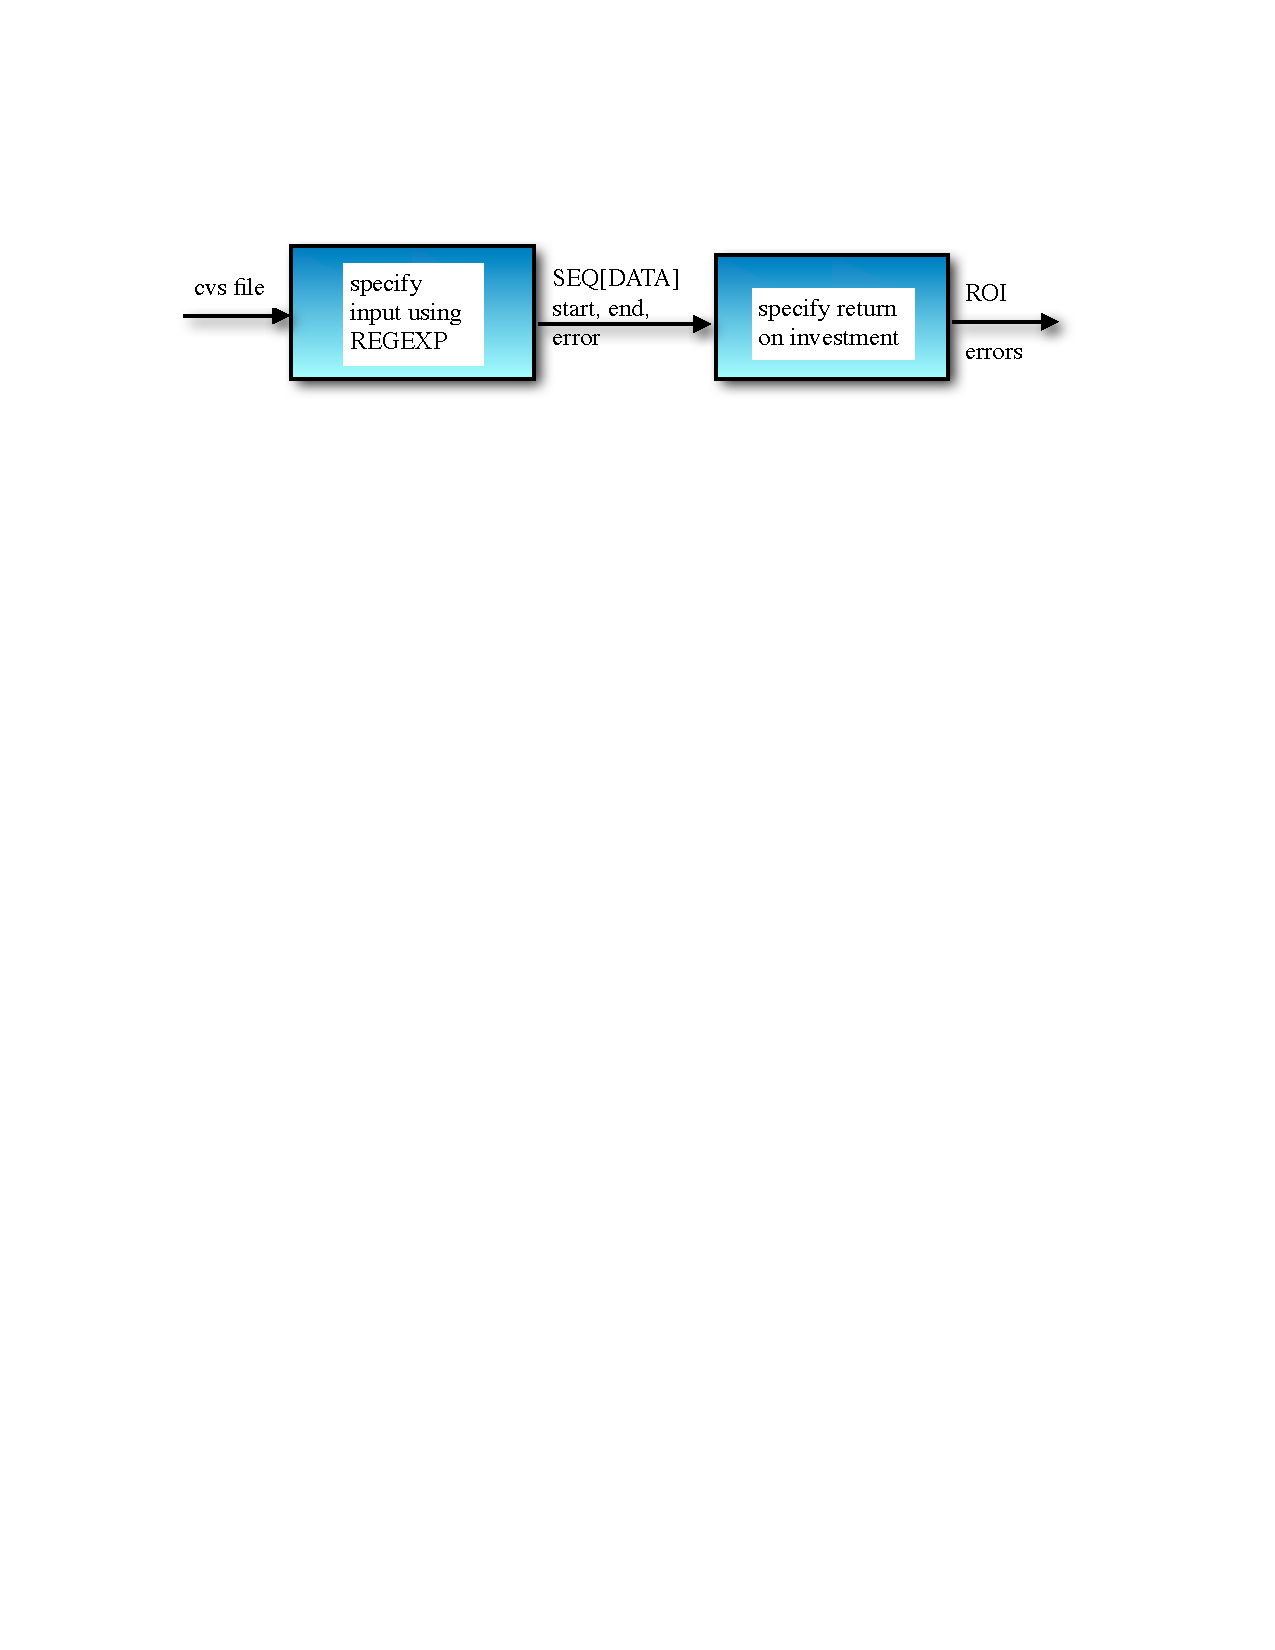
\includegraphics[scale=0.8]{inputs/spec.pdf}
%\begin{figure}
\resizebox{\textwidth}{!}
{
\def\data{type DATA}
\def\input{type input-csv}
\def\roi{type roi}
\def\control{module control}
\renewcommand\tikzumlfillclasscolor{white}
\def\do{\quad\textbf{do}~} %%Needed
\centering
\resizebox{\textwidth}{!}{\begin{tikzpicture}

\umlclass{\data}
{
\use DATE\comment see appendix B\\
\cset $DATA \eqdef$\\
$\qquad  Data(date: DATE, mv:\Fl, cf:\Fl, af:\Fl,bench: \Fl\bunion\{Void\})$\\
$\qquad$\require $valid\_date(date)$\\

}
{
\comment the above declaration induces an injective function with accessors\\
$Data: DATE \cprod \Fl \cprod \Fl \cprod \Fl \cprod \Fl\bunion\{Void\} \tinj DATA$\\
\const $mv,cf,af : DATA \tfun \Fl$\\
\comment market-value, cash-flow and agent-fees\\
\const $bench: DATA \tfun \Fl\bunion\{Void\}$\comment benchmark\\
\axiom $\forall d:DATA \itholds d=Data(date(d),mv(d),cf(d),bench(d))$\\
\comment e.g. $DATA = \{ Data(\squote{2007-02-11},105000,15000,0,Void), \cdots\}$
}
        
\umlclass[x=-4.5, y=-6.4]{\input}
{
\use type $REGEXP, DATA$ \\
\textbf{param} $csvfile : \St$\\
\comment input parameter\\
\query $tr : SEQ[DATA]$\\
\comment sequence of transactions\\
\require $csvfile  \in VALID\_FILE$\\
$\query start, end: DATE$\\
\require $csvfile  \in VALID\_FILE$\\
}
{
\comment see Fig.~\ref{fig:input} for the details
}
        
\umlclass[x=4.5, y=-6.4]{\roi}
{
\use $input(cvsfile)$\\
\param $cvsfile:\St$\\
\query $report:\St$
}
{
\comment see function table for outputs\\
}
        
\umlclass[y=-12.4]{\control}
{
\comment specification pattern for transfomational programs
}
{
\event $roiReport \leftarrow invoke$\\
\any $file:\St$\\
$\quad$\use $roi(file)$ \textbf{as} $r$\\
\ddo $roiReport := r.report$\\\\
\comment dynamic use of module \textbf{roi}\\
\comment instantiate $cvsfile$ as $file$

}
        
\umlunicompo{\input}{\data}
\umlunicompo{\roi}{\data}
\umlunicompo{\roi}{\input}
\umlunicompo{\control}{\roi}
\end{tikzpicture}}
}
%\end{figure}
\caption{Module specification of return on investment}
\end{figure}

\begin{figure}
\resizebox{\textwidth}{!}{{\begin{tikzpicture}
\renewcommand\tikzumlfillclasscolor{white}
\umlclass{type input-csv}
{
\use type $REGEXP, DATA, DATE$ 
\comment we let $\epsilon = \{``"\}$, eol = $\{``\backslash\textrm{n}"\}$ etc.\\
\cset $DATA \eqdef Data(date: DATE, mv:\Fl, cf:\Fl, af:\Fl,bench: \Fl\bunion\{Void\})$\\
\textbf{param} $csvfile : \St$\comment input parameter\\
\query $tr : SEQ[DATA]$\comment sequence of transactions defined by axiom below\\
\require $csvfile  \in VALID\_FILE$\\
$\query start, end: DATE$\\
\require $csvfile  \in VALID\_FILE$\\
}
{
\const $VALID\_FILE : \regexp$\\
$\eqdef HEADER \cdot PARAMETERS \cdot \textrm{eol} \cdot ROW \cdot \textbf{*}(\textrm{eol} \cdot ROW)\cdot \textbf{*}(``,"|\textrm{eol})$\\
\const $HEADER: REGEXP$\\
$\eqdef \textbf{*} (HLINE \cdot eol) $\\
\const $HLINE:REGEXP$\\
$\eqdef \textbf{*} (\Sigma \backslash \textrm{eol}) \backslash (EV\_PER\cdot \textbf{*} \Sigma)$\\
\const $PARAMETERS:REGEXP$\\
$\eqdef EV\_PER \cdot DATE\_STR \cdot``\_ \textrm{to}\_" \cdot DATE\_STR \cdot \textbf{*}``,"\cdot \textrm{eol}\cdot COL\_HEAD$\\
\const $COL\_HEAD:REGEXP$\\
$ \eqdef +``," \cdot eol \cdot$\\ $\qquad``\textrm{Transaction\_Date,Market\_Value,Cash\_Flow,Agent\_Fees,Benchmark}"\cdot\textbf{*} ``,"$\\
\const $EV\_PER:REGEXP \eqdef ``\textrm{Evaluation\_Period:\_}" $\\
\const $ROW: \regexp$\\
$\eqdef (DATE\_STR \cdot ``,"\cdot  FLOAT\cdot ``,"  \cdot (FLOAT|\epsilon) \cdot ``," \cdot (FLOAT|\epsilon)\cdot$\\
$\qquad ``,"  \cdot (FLOAT\cdot``\%"|\epsilon)\cdot \textbf{*}``,")$\\
\const $s2d : DATE\_STR \tfun DATE$\comment see birthday book for $DATE$\\
\const $s2f: FLOAT \tfun \Fl$\comment deferred, $FLOAT$ is the string version of $\Fl$\\
\const $f2s : \Fl \tfun FLOAT$\comment deferred, see your favourite programming language\\
\const $d2s : DATE \tfun DATE\_STR$\comment deferred\\
\const $s2optf[G]: (FLOAT | \epsilon)\cprod G\tfun  \Fl \bunion G$\comment string-to-optional float \\
\where $\forall G \itholds s2optf \in (FLOAT | \epsilon)\cprod G\tfun  \Fl \bunion G$\\
\comment parameter $G$ is a set such as $\{Void\}$ or a default value such as $\{0\}$\\
\const $f : ROW \tfun DATA$\\
\textbf{dummy} $w:ROW$ and $s_0, s_1, s_2,s_3:\St$\\
\axiom 1:\comment definition of function $f$ that maps a row string to data\\
$\qquad\qquad w \in  (d2s(d)\cdot ``,"\cdot s_0 \cdot ``,"\cdot s_1 \cdot ``,"\cdot s_2 \cdot ``," \cdot s_3 \cdot \textbf{*}``,") $ \\ 
$\qquad ~~\land ~ (s_4 \cdot ``\%" = s_3 \lor s_4 = s_3 = \epsilon)$ \\
$\qquad \implies   f (w) = Data(d, s2f(s_0), s2optf(s_1,0), s2optf(s_2,0), s2optf(s_4,\text{Void}))$\\
\query $error : \Bl \eqdef textfile \not\in VALID\_FILE$\comment definition of $tr,start,end$\\
\axiom 2: \comment definition of $tr,start, end$\\
$\qquad\qquad csvfile  \in VALID\_FILE \implies$\\
$\qquad\qquad (\exists h,foot,s,e: \St; data:SEQ[ROW]$\\
$\qquad\qquad~~|~~~ h\in HEADER \cdot EV\_PER \cdot s \cdot``\_ \textrm{to}\_" \cdot e \cdot \textbf{*}``,"\cdot \textrm{eol}\cdot COL\_HEAD$\\
$\qquad\qquad~~~ \land data \in SEQ[ROW]$\\
$\qquad\qquad~~~ \land end \in \textbf{*}(\squote{,}|eol)$\\
$\qquad\qquad~~~ \land textfile \in h \cdot (\cdot i| 0 \leq i < \#data \itholds eol \cdot data(i)) \cdot foot$\\
$\qquad\qquad~ \itholds~~~ tr = (\cdot i | 0 \leq i < \#data \itholds <f(data(i))>$\\
$\qquad\qquad\qquad \land (start=s2d(s)) \land (end = s2d(e))$\\
$\qquad\qquad)$\\
}
\end{tikzpicture}
}
}
\caption{Type input-csv}
\label{fig:input}
\end{figure}

\newpage
%%%%%%%%%%%%%%%%%%%%%%%%%%%%%%%%%%%%%%%%%%%
%%%%%%%%%%%%%%%%%%%%%%%%%%%%%%%%%%%%%%%%%%%
%%%%%%%%%%%%%%%%%%%%%%%%%%%%%%%%%%%%%%%%%%%
%%%%%%%%%%%%%%%%%%%%%%%%%%%%%%%%%%%%%%%%%%%
\newcommand{\tab}{\hspace*{2em}}

{
\centering
\begin{longtable}{|l|}

\hline
\multicolumn{1}{|c|}{\textbf{TWR\_ROI\_CALCULATION}}\\

\hline
\textbf{\comment input} (\textit{input.csv})\\
\\
\textit{tr}: SEQ[DATA]\\
\comment sequence of data [\textit{date, market\_value, cash\_flow, agent\_fees, benchmark}]\\
\comment \textit{tr.domain} = \{1,2,...,\textit{tr.count}\}\\
\\
\textit{count}: INTEGER$\eqdef$\textit{tr.count}\\
\\
\textit{dates}: SET[DATE]$\eqdef$\{\textit{t $\in$ tr$\itholds$t.date}\}\\
\\
$start:$ DATE $\eqdef tr[1]$ \comment first date of the file\\
$end:$ DATE $\eqdef tr[count]$ \comment last date of the file\\ 
\\
\textit{duration}: VALUE$\eqdef$ \textit{days(end - start)}$\div$(365.2422) \\
\comment years between \textit{start} and \textit{end} calculated by days\\
\comment \textit{days}(x) similar to Excel\\

\\
\\
\textbf{\comment output calculation} (\textit{input.out.csv})\\
\\
\textit{di (d}:DATE): INTEGER\\
\comment index into sequence of transaction for date \textit{d}\\
\require \textit{d $\in$ dates} \\
\ensure \textit{Result $\in$ tr.domain $\land$ tr[Result].date=d}\\
\\

TODO: DANS REQUIRE I VARIE DANS L'INTERVALLE D'INDICE\\
 DEFINIT PAR S ET E\\
IL FAUT VERIFIER QUE CE SOIT BIEN CA DANS LES E/R\\
\comment TWR for the period \textit{s .. e}\\
\textit{twr (s, e}: DATE): VALUE\\
\require\\
	\tab \textit{s, e $\in$ dates}\\
	\tab \textit{e $>$ s}\\
	\tab \textit{$\forall$i $\in$ di(s)+1..di(e)$\itholds$tr[i-1].mv + tr[i-1].cf + tr[i-1].af $\neq$ 0}\\
\ensure\\
	\tab \textit{Result $\eqdef$ ($\Pi$i:INTEGER $|$ di(s) $<$i$\le$ di(e)$\itholds$wealth(i)) - 1}\\
	\tab where \textit{wealth(i) $\eqdef$ tr[i].mv$\div$(tr[i-1].mv + tr[i-1].cf + tr[i-1].af)}\\
\\

TODO: SUPPRIMER LA VARIABLE DURATION ET\\
 REMPLACER PAR LA BONNE CHOSE\\
\textit{annual\_compounded\_TWR (s, e}: DATE): VALUE \\
\ensure \\
	\tab \textit{(duration$\ge 1)\Rightarrow Result=((1+twr(s, e))^{1\div duration}-1)*100$}\\
	\tab \textit{(duration$<$1)$\Rightarrow$ Result= twr(s, e) * 100}\\
\\

TODO: IL FAUT RETIRER DES E-R DESCRIPTION QUE\\
 AF EST UN DEPOSIT AILLEUR QUE POUR LE TWR\\
TODO:VERIFIER QUE LE + POUR LES AGENT FEES\\
 CI DESSOUS EST CORRECT,DANS LE CODE JE L'AI\\
CHANGE EN -\\
\textit{roi (s, e}: DATE): VALUE\\
\require\\
	\tab \textit{s, e $\in$ dates}\\
	\tab\textit{e $>$ s}\\
\ensure\\
	\tab \textit{(tr[m].mv+tr[m].cf) $\ast (1+Result\div 100)^{days(e - s)\div365.2422}$ }\\
	\tab \tab \textit{+ ($\Sigma i  |  m <i<n\itholds (tr[i].cf + tr[i].af) \ast $}\\
	\tab \tab \textit{$(1+Result\div 100)^{days(e - tr[i].date)\div365.2422}) - tr[n].mv = 0$}\\
\where \\
	\tab \textit{m = di(s)}\\ 
	\tab \textit{n = di(e)}\\
\\
\\

$year(d:$ DATE): INTEGER\\
\require\\
\tab $d = "yyyy - mm - dd"$\\
\ensure\\
\tab $Result = yyyy$\\
\\	

$mon(d:$ DATE): INTEGER\\
\require\\
\tab $d = "yyyy - mm - dd"$\\
\ensure\\
\tab $Result = mm$\\
\\	

$day(d:$ DATE): INTEGER\\
\require\\
\tab$ d = "yyyy - mm - dd"$\\
\ensure\\
\tab $Result = dd$\\
\\	

TODO FAIRE LES FONCTION TABLE POUR MIN ET MAX\\
TODO VOIR POUR LE REQUIRE DE MIN ET MAX\\
$\uparrow$ ($f, s$: DATE): DATE\\
\require\\
\ensure\\
\tab $<<$ see table...$>>$\\
\\
$\downarrow$ ($f, s$: DATE): DATE\\
\require\\
\ensure\\
\tab $<<$ see table...$>>$\\
\\
TODO FAIRE ET NUMEROTER LA FUNCTION TABLE\\
 DE LA FCT SUIVANTE\\
\textit{at (d}: DATE): DATA\\
\ensure\\
\tab $<<see$ $table ... >>$ \\
\\

TODO: FAIRE UN CHECK AVANT (DANS LE MAIN)\\
POUR SAVOIR SI S ET E SONT DANS DATES\\
\textit{bm\_calculable (s, e}: DATE): $\Bool$\\
\require\\
	\tab $s, e \in dates$\\ 
	\tab $s \neq e$\\
	\tab $s < e$\\
\ensure\\
\tab $Result = at[end\downarrow a].bench \neq void $\\
\tab \tab $\wedge (\forall d \in DATE | mon(d) = day(d) = 1 \wedge year(s) < year(d) \le year(e)$\\
\tab \tab \tab $\itholds at[d].bench \neq void)$\\
\tab \tab $\wedge ((C \wedge at[e].bench \neq void) \vee (\neg C \wedge at[end \downarrow b].bench \neq void))$\\
\where\\
\tab $a = "year(s)+1 - 01 - 01"$\\
\tab $b = "year(e)+1 - 01 - 01"$\\
\tab $C = (mon(e) = 1 \wedge day(e) = 1)$\\
\\

TODO RAJOUTER LA FUNCTION TABLE\\
\comment the function below return a set of DATA with a benchmark $\neq$ void\\
\textit{bm\_seq (s, e}: DATE): SEQ[DATA]\\
\require\\
\tab $s,e\in$ $dates$\\
\tab \textit{bm\_calculable(s, e) }\\
\ensure\\
	\tab $Result = (\oplus i | di(s)<i < di(e) \wedge tr[i].bench \neq void \itholds <tr[i]>)$\\
	\tab \tab $ \oplus <t>$\\

\where\\
\tab t = $<<$ see table ...$>>$\\
\\

$po(s,e, d1, d2:$ DATE) : VALUE\\
\require\\
	\tab $d1 \neq d2 $ \\
\ensure\\
	\tab $Result \eqdef days(d2 \downarrow e - d1 \uparrow s) \div days(d2 - d1)$\\
\\
 
$bm\_final\_value(s,e:$ DATE): VALUE\\
\require\\
\tab $s, e \in dates$\\
\tab $bm\_calculable(s,e) $\\
\ensure\\
\tab $Result \eqdef$\\
\tab $tr[m].mv \ast (\Pi i, seq, t| seq = bm\_seq(s, e) \wedge a \oplus seq \wedge 1 \le i \le \# seq$\\
  \tab \tab $\wedge t = seq[i] \itholds t.bench^{po(s, e, seq[i-1].date, t.date)} )$\\
\tab $+ (\Sigma k | m \le k < n \itholds (tr[k].cf - tr[k].af) \ast$\\
\tab \tab $(\Pi i,seq,t | seq = bm\_seq(tr[k].date, e) \wedge b(k) \oplus seq \wedge1 \le i \le \# seq$\\
\tab \tab $\wedge t = seq[i] \itholds t.bench^{po(s, e, seq[i-1].date, t.date)}))$\\
\where\\
\tab $m = di(s)$\\
\tab $n = di(e)$\\
{\hspace*{1em}} \comment $a$ defines seq[0] in the first product\\
{\hspace*{1em}} \comment $b(k)$ defines seq[0] in the second product\\
\tab$a = <("year(s) - 01 - 01", 0, 0, 0, void)>$\\
\tab$b(k) = <("year(tr[k].date) - 01 - 01", 0, 0, 0, void)>$ \\
\\

EST-CE QUE C'EST NORMAL QU'IL N'Y AI PAS DE AF DANS \\
BENCHMARK?\\
$benchmark (s, e$: DATE): VALUE\\
\require\\
\tab $s, e \in dates$\\
\tab $bm\_calculable(s, e)$\\
\ensure\\
\tab $tr[m].mv \ast (1+Result \div 100)^{days(e-s)\div365.2422}) $\\
\tab $+ (\Sigma k | m \le k < n \itholds tr[k].cf \ast$\\
\tab \tab $(1+Result \div 100)^{days(e - tr[k].date)\div365.2422}) - FV= 0$\\
\where\\
\tab $m = di(s)$\\
\tab $n = di(e)$\\
\tab $FV \eqdef bm\_final\_value(s,e) $\\
\\


\hline
\textbf{Invariants}\\
\\
(1) \textit{ (start$<$end)$\wedge$(start,end$\in$dates)} \\
\comment metadata evaluation period is in range and valid\\
\\
(2) \textit{$\forall$t$\in$tr$\itholds$t.date$\neq$Void$\wedge$t.mv$\ge$0}\\
\comment every row has a date and a non-negative market value\\
\\
(3) \textit{$\forall$i$\in$2..count$\itholds$tr[i].date$>$tr[i-1].date}\\
\comment date are unique and ordered\\
\\
(4) \textit{$\forall$t$\in$tr$\itholds$t.mv+t.cf$\ge$0}\\
\comment Cannot withdraw more than the market value\\
\\
(5) \textit{$\forall$i$\in$2..count $|$ tr[i-1].mv=0$\wedge$tr[i-1].cf=0$\itholds$tr[i].mv=0}\\
\comment account coannot grow from zero market value and cash flow\\

\hline
\caption{Mathematical model for the ROI system}
\label{tab:twr_calculation}
\end{longtable}
}


%%%%%%%%%%%%%%%%%%%%%%%%%%%%%%%%%%%%%%%%%%%
%%%%%%%%%%%%%%%%%%%%%%%%%%%%%%%%%%%%%%%%%%%
%%%%%%%%%%%%%%%%%%%%%%%%%%%%%%%%%%%%%%%%%%%
%%%%%%%%%%%%%%%%%%%%%%%%%%%%%%%%%%%%%%%%%%%


%%%%%%%%%%%%%%%%%%%%%%%%%%%%%%%%%%%%%%%%%

\bibliographystyle{plain}
\bibliography{inputs/ref}

TODO : A CHECKER !!! + TITRE

\begin{table}[H]
{
\centering

\begin{tabular}{|l|l|l||l|l|}
\hline
\multicolumn{3}{|l||}{fi, se : DATE} & Min & Max\\ 

\hline
\multicolumn{3}{|l||}{year(fi) $<$ year(se)} & fi & se\\ 

\hline
\multicolumn{3}{|l||}{year(fi) $>$ year(se)} & se & fi\\ 

\hline
year(fi) $=$ year(se) & \multicolumn{2}{|l||}{mon(fi) $<$ mon(se)} & fi & se\\ 

\cline{2-5}
& \multicolumn{2}{|l||}{mon(fi) $>$ mon(se)} & se & fi\\

\cline{2-5}
& mon(fi) $=$ mon(se) & day(fi) $<$ day(se) & fi & se\\

\cline{3-5}
& & day(fi) $\ge$ day(se) & se &  fi\\

\hline
\end{tabular}

\caption{Function table for ROI system (calculation of the benchmarks)}
\label{table:ftable_bench}
}
\end{table}
%%%
\begin{table}[H]
{
\centering

\begin{tabular}{|l|l||l|}
\hline
\multicolumn{2}{|c||}{} & at(d)\\ 

\hline
\multicolumn{2}{|l||}{d$\in$dates} & $\exists$! i $|$ 1$\le$i$\le$count$\itholds$Result = tr[i]$\wedge$Result.date = d\\ 

\hline
d$\notin$dates & mon(d)=1 $\wedge$ day(d)=1 & Result = (d,0,0,0,void)\\

\cline{2-3}
& $\lnot$(mon(d)=1 $\wedge$ day(d)=1) & null\\

%\hline
%Valid$\_$CSV & $\lnot$(Start$\_$Valid) $\vee$ & |& W & | & |\\ 
%& $\lnot$(End$\_$Valid) $\vee$ &&&&\\
%& end $\le$ start &&& &\\
%
%\cline{2-6}
%& Start$\_$Valid  $\wedge$ & |& | & roi(first,last) & roi(start,end)\\
%& End$\_$Valid $\wedge$ &&&&\\
%& end$>$start &&&&\\
%
%\hline
%\multicolumn{2}{|l||}{Invalid$\_$CSV} & E & |& | & |\\ 
%
\hline
\end{tabular}

\caption{Function table for ROI system (calculation of the ROIs)}
\label{table:ftable_ROI}
}
\end{table}

%%%




\newpage

%%%%%%%%%%%%%%%%%%%
\subsection{Function tables}




\subsubsection{Abbreviations, conditions and messages}
{\centering
\begin{longtable}{|l|p{11cm}|}
\hline
\textbf{Abbreviation} & \textbf{Description}\\

\hline
first & tr[1].date \\

\hline
last & tr[tr.count].date\\

\hline
 a\_c\_TWR & annual\_compounded\_TWR\\
& (see TWR\_ROI\_CALCULATION (Fig.~\ref{tab:twr_calculation})) \\

\hline
 b & benchmark (see TWR\_ROI\_CALCULATION (Fig.~\ref{tab:twr_calculation}))\\



\hline
\end{longtable}

\centering
\begin{longtable}{|l|p{12cm}|}
\hline
\textbf{Condition} & \textbf{Description}\\

\hline
C1 & \textit{$\forall$i $\in$ 2..count$\itholds$tr[i-1].mv + tr[i-1].cf + tr[i-1].af $\neq$ 0}\\

\hline
C2 & \textit{$\forall$i $\in$ di(start)+1..di(end)$\itholds$tr[i-1].mv + tr[i-1].cf + tr[i-1].af $\neq$ 0}\\

\hline
C3 & benchmark\_calculable(first,last)\\
& (see TWR\_ROI\_CALCULATION (Fig.~\ref{tab:twr_calculation}))\\

\hline
C4 & benchmark\_calculable(start,end)\\
&(see TWR\_ROI\_CALCULATION (Fig.~\ref{tab:twr_calculation}))\\

\hline
 Start\_Valid & (start $\in$ dates$\cup$\{null\}) $\wedge$ (start in ISO format)\\
& (if Start\_Valid $\wedge$ start=null, then start=tr[1].date)\\

\hline
 End\_Valid & (end $\in$ dates$\cup$\{null\}) $\wedge$ (end in ISO format)\\
&(if End\_Valid $\wedge$ end=null, then end=tr[tr.count].date)\\

\hline
Name & (csvfile.name = null)\\

\hline
\end{longtable}

\centering
\begin{longtable}{|l|p{13cm}|}
\hline
\textbf{Message} & \textbf{Description}\\

\hline
 E & "Invalid file"\\

\hline
W & "Invalid evaluation period"\\

\hline
W1 & "The TWR for the whole input is not calculable"\\

\hline
W2 & "The TWR's are not calculable"\\

\hline
W3 & W + W1\\

\hline
W4 &  "Benchmark for the whole input is not calculable"\\

\hline
W5 & "The benchmarks are not calculable"\\

\hline
W6 & W + W4\\

\hline
W7 & "Incomplete file: absence of name"\\

\hline

\end{longtable}
}

\begin{landscape}
\subsubsection{Calculation of the TWRs}

\begin{table}[H]
{
\centering
\begin{tabular}{|l|l|l|l||l|l|l|l|}
\hline
\multicolumn{4}{|c||}{} & Error & Warning &TWR & TWR\\ 
\multicolumn{4}{|l||}{}&&& (whole input) & (evaluation period)\\

\hline
Valid$\_$CSV & $\lnot$(Start$\_$Valid) $\vee$ & \multicolumn{2}{|l||}{C1} & | & W & a\_c\_TWR(first,last) & |\\ 
& $\lnot$(End$\_$Valid) $\vee$& \multicolumn{2}{|l||}{} &&& &\\
& end $\le$ start & \multicolumn{2}{|l||}{} &&& &\\

\cline{3-8}
& & \multicolumn{2}{|l||}{$\lnot$C1} & | & W3 & | & |\\ 


\cline{2-8}
& Start$\_$Valid  $\wedge$  & \multicolumn{2}{|l||}{C1} & | & | & a\_c\_TWR(first,last) & a\_c\_TWR(start,end)\\ 
& End$\_$Valid $\wedge$  & \multicolumn{2}{|l||}{} &&&&\\
& end$>$start   & \multicolumn{2}{|l||}{}&&&&\\

\cline{3-8}
&& $\lnot$C1 & C2 & | & W1 & | & a\_c\_TWR(start,end)\\

\cline{4-8}
&& & $\lnot$C2 & | & W2 & | & |\\

\hline
\multicolumn{4}{|l||}{Invalid$\_$CSV} & E & | & | & |\\ 

\hline
\end{tabular}

\caption{Function table for ROI system (calculation of the TWRs)}
\label{table:ftable_TWR}
}
\end{table}
\end{landscape}


%%%



\begin{landscape}
\subsubsection{Calculation of the ROIs}

\begin{table}[H]
{
\centering

\begin{tabular}{|l|l||l|l|l|l|}
\hline
\multicolumn{2}{|c||}{} & Error & Warning & ROI (whole input) & ROI (evaluation period)\\ 

\hline
Valid$\_$CSV & $\lnot$(Start$\_$Valid) $\vee$ & |& W & | & |\\ 
& $\lnot$(End$\_$Valid) $\vee$ &&&&\\
& end $\le$ start &&& &\\

\cline{2-6}
& Start$\_$Valid  $\wedge$ & |& | & roi(first,last) & roi(start,end)\\
& End$\_$Valid $\wedge$ &&&&\\
& end$>$start &&&&\\

\hline
\multicolumn{2}{|l||}{Invalid$\_$CSV} & E & |& | & |\\ 

\hline
\end{tabular}

\caption{Function table for ROI system (calculation of the ROIs)}
\label{table:ftable_ROI}
}
\end{table}
\end{landscape}

%%%


\begin{landscape}
\subsubsection{Calculation of the benchmarks}

\begin{table}[H]
{
\centering

\begin{tabular}{|l|l|l|l||l|l|l|l|}
\hline
\multicolumn{4}{|c||}{} & Error & Warning & Benchmark & Benchmark\\ 
\multicolumn{4}{|l||}{}&&&(whole input) & (evaluation period)\\


\hline
Valid$\_$CSV & $\lnot$(Start$\_$Valid) $\vee$ & \multicolumn{2}{|l||}{C3} & | & W & b(first,last) & |\\ 
& $\lnot$(End$\_$Valid) $\vee$& \multicolumn{2}{|l||}{} &&& &\\
& end $\le$ start & \multicolumn{2}{|l||}{} & &&&\\

\cline{3-8}
& & \multicolumn{2}{|l||}{$\lnot$C3}& | & W6 & | & |\\ 

\cline{2-8}
& Start$\_$Valid  $\wedge$  & \multicolumn{2}{|l||}{C3} & | & | & b(first,last) & b(start,end)\\ 
& End$\_$Valid $\wedge$  & \multicolumn{2}{|l||}{} &&&&\\
& end$>$start   & \multicolumn{2}{|l||}{}&&&&\\

\cline{3-8}
&& $\lnot$C3 & C4 & | & W4 & | & b(start,end)\\

\cline{4-8}
&& & $\lnot$C4 & | & W5 & | & |\\

\hline
\multicolumn{4}{|l||}{Invalid$\_$CSV} & E & |& |& |\\ 

\hline
\end{tabular}

\caption{Function table for ROI system (calculation of the benchmarks)}
\label{table:ftable_bench}
}
\end{table}
\end{landscape}

%%%

\subsubsection{Name of the portfolio history}

\begin{table}[H]
{
\centering

\begin{tabular}{|l||l|}
\hline
 & Warning\\ 

\hline
Name  & |\\ 

\hline
$\lnot$Name & W7 \\ 

\hline
\end{tabular}

\caption{Function table for ROI system (name of the portfolio history)}
\label{table:ftable_name}
}
\end{table}




\section{Acceptance tests}

\bigskip
{\centering
\begin{tabular}{|p{1.2in}|p{4in}|}
\hline
\textbf{Test Case ID} & T1 - test\_date\_invalid.csv \\ 
\hline
\textbf{Description} & Verify that an invalid date raises an error.\\
\hline
\textbf{Requirement IDs tested} & R3.1 \\ 
\hline
\textbf{Type} & Negative \\ 
\hline
\textbf{Initial State} & A directory containing the CSV file.\\
\hline 
\textbf{Action} & Execute the ROI system on the CSV file \\
\hline 
\textbf{Consequences} & Output : "Error: Invalid file." \\ 
\hline
\end{tabular}
%%%%
\bigskip\bigskip
\centering
\begin{tabular}{|p{1.2in}|p{4in}|}
\hline
\textbf{Test Case ID} & T2 - test\_date\_invalid\_February.csv \\ 
\hline
\textbf{Description} & Verify that an invalid date (because of the leap years) raises an error.\\
\hline
\textbf{Requirement IDs tested} & R3.1 \\ 
\hline
\textbf{Type} & Negative \\ 
\hline
\textbf{Initial State} & A directory containing the CSV file.\\
\hline 
\textbf{Action} & Execute the ROI system on the CSV file \\
\hline 
\textbf{Consequences} & Output : "Error: Invalid file." \\ 
\hline
\end{tabular}
%%%%
\bigskip
\centering
\begin{tabular}{|p{1.2in}|p{4in}|}
\hline
\textbf{Test Case ID} & T3 - test\_tuple\_without\_date.csv \\ 
\hline
\textbf{Description} & Verify that a tuple without a date raises an error.\\
\hline
\textbf{Requirement IDs tested} & E5.5 - R3.1 \\ 
\hline
\textbf{Type} & Negative \\ 
\hline
\textbf{Initial State} & A directory containing the CSV file.\\
\hline 
\textbf{Action} & Execute the ROI system on the CSV file \\
\hline 
\textbf{Consequences} & Output : "Error: Invalid file." \\ 
\hline
\end{tabular}
%%%%
\bigskip
\centering
\begin{tabular}{|p{1.2in}|p{4in}|}
\hline
\textbf{Test Case ID} & T4 - test\_negative\_market\_value.csv \\ 
\hline
\textbf{Description} & Verify that a negative market value raises an error.\\
\hline
\textbf{Requirement IDs tested} & E5.5 - R3.1 \\ 
\hline
\textbf{Type} & Negative \\ 
\hline
\textbf{Initial State} & A directory containing the CSV file.\\
\hline 
\textbf{Action} & Execute the ROI system on the CSV file \\
\hline 
\textbf{Consequences} & Output : "Error: Invalid file." \\ 
\hline
\end{tabular}
%%%%
\bigskip
\centering
\begin{tabular}{|p{1.2in}|p{4in}|}
\hline
\textbf{Test Case ID} & T5 - test\_dates\_non\_unique.csv \\ 
\hline
\textbf{Description} & Verify that two tuples with the same date raise an error.\\
\hline
\textbf{Requirement IDs tested} & E5.6 - R3.1 \\ 
\hline
\textbf{Type} & Negative \\ 
\hline
\textbf{Initial State} & A directory containing the CSV file.\\
\hline 
\textbf{Action} & Execute the ROI system on the CSV file \\
\hline 
\textbf{Consequences} & Output : "Error: Invalid file." \\ 
\hline
\end{tabular}
%%%%
\bigskip
\centering
\begin{tabular}{|p{1.2in}|p{4in}|}
\hline
\textbf{Test Case ID} & T6 - test\_dates\_non\_ordered.csv \\ 
\hline
\textbf{Description} & Verify that tuples which are not ordered raise an error.\\
\hline
\textbf{Requirement IDs tested} & E5.6 - R3.1 \\ 
\hline
\textbf{Type} & Negative \\ 
\hline
\textbf{Initial State} & A directory containing the CSV file.\\
\hline 
\textbf{Action} & Execute the ROI system on the CSV file \\
\hline 
\textbf{Consequences} & Output : "Error: Invalid file." \\ 
\hline
\end{tabular}
%%%%
\bigskip
\centering
\begin{tabular}{|p{1.2in}|p{4in}|}
\hline
\textbf{Test Case ID} & T7 - test\_withdraw.csv \\ 
\hline
\textbf{Description} & Verify that a withdraw which is greater that the market value raises an error.\\
\hline
\textbf{Requirement IDs tested} & E5.7 - R3.1 \\ 
\hline
\textbf{Type} & Negative \\ 
\hline
\textbf{Initial State} & A directory containing the CSV file.\\
\hline 
\textbf{Action} & Execute the ROI system on the CSV file \\
\hline 
\textbf{Consequences} & Output : "Error: Invalid file." \\ 
\hline
\end{tabular}
%%%%
\bigskip
\centering
\begin{tabular}{|p{1.2in}|p{4in}|}
\hline
\textbf{Test Case ID} & T8 - test\_grow.csv \\ 
\hline
\textbf{Description} & Verify that an account which grow from zero market value and cash flow raises an error.\\
\hline
\textbf{Requirement IDs tested} & E5.8 - R3.1 \\ 
\hline
\textbf{Type} & Negative \\ 
\hline
\textbf{Initial State} & A directory containing the CSV file.\\
\hline 
\textbf{Action} & Execute the ROI system on the CSV file \\
\hline 
\textbf{Consequences} & Output : "Error: Invalid file." \\ 
\hline
\end{tabular}
}







\section{Requirements Traceability matrix}

\begin{tabular}{|p{1.5in}|p{3.5in}|}
\hline
\textbf{Requirement ID}	 & \textbf{Test Case IDs}\\ 
\hline
R3.1 & T1, T2, T3, T4, T5, T6, T7, T8\\
\hline
\end{tabular}




\newpage
\appendix

\section{REGEXP}


A set of strings is used as the model for regular expressions. We use prefix operators for the Kleene closure (e.g. $*x$ where $x$ is a regular expression such as $\{\squote{hello}\}$) and iteration at least one or more (e.g. $\textrm{+}x$) rather than suffix operators. Note that where there is no confusion we use \squote{hello} instead of $\{\squote{hello}\}$ where the set is a singleton. 

We may use type REGEXP to specify a $FLOAT\_STRING$ as follows.

\begin{align}
FLOAT\_STRING = &\squote{+}Inf\\
&|\squote{-}Inf\\
&|NaN\\
&|(\squote{-}|\squote{+}|\epsilon)\cdot(^*d\cdot\squote{.}|\epsilon)\cdot
	^*\!\!d\cdot ((\squote{e}\cdot(\squote{-}|\epsilon)\cdot^\textrm{+}d)\,|\,\epsilon)\\
d = &\squote{0} | \squote{1} | \cdots |\squote{9} 
\end{align}

In the above we use the convention that \squote{e}, for example, really stands for the single set $\{\squote{e}\}$.


\begin{figure} [H]
\resizebox{\textwidth}{!}
{
\begin{tikzpicture}
\renewcommand\tikzumlfillclasscolor{white}
\umlclass{type REGEXP}
{
\cset $\regexp$\comment set of all regular string expressions\\
\axiom $\regexp \subseteq \pow(\St)$\\
\cset $\Sigma \eqdef \{``0", ``1",  ``2", \cdots, ``a", ``b",  \textrm{ etc., all printing characters} \}$\\
}
{

\dummy $x,y,z : \regexp$\\
\dummy $s,t,u : \St$\\

\axiom $\forall s\in\Sigma \itholds \{s\} \in \regexp$\\

\const $0:\regexp \eqdef \{\}$\comment zero is the unit element of alternation\\
\const $1:\regexp\eqdef \{``"\}$\comment $1$ is the unit element of concatenation\\
\comment we also use $\epsilon$ instead of $1$\\

\const \infix $``|": \regexp \cprod \regexp \tfun \regexp$\\
\comment alternation\\
\const \infix $``\cdot": \regexp \cprod \regexp \tfun \regexp$\\
\comment concatenation\\

\const \prefix$``*": \regexp \cprod \regexp \tfun \regexp$\\
\comment iteration zero or more times\\
\const \prefix$``\textrm{+}": \regexp \cprod \regexp \tfun \regexp$\\
\comment iteration one or more times\\

\axiom $s \in x|y ~\equiv~ s\in x \,\lor\, s\in y$\\
\theorem $x | 0 = 0 | x = x$\\
\axiom $s \in x\cdot y ~\equiv~ (\exists t,u| s=t\cdot u \itholds t\in x \land u\in y)$\\
\comment note that $t\cdot u$ is concatenation over $SEQ[\St]$\\
\theorem $1 \cdot x ~=~ x \cdot 1 ~=~ 1$\
\comment 1 is the identity of concatenation\\

\const \infix ``\^{}"$: \regexp \cprod \nat \tfun \regexp$\\
\comment use this operator by raising the second argument like an exponent\\
\axiom $x^n = (\cdot i\suchthat 0 \leq i \leq n \itholds x)$\comment concatenation quantifier\\

\comment e.g. $x^3 = x \cdot x \cdot x$\\
\theorem $x^0 = 1$\\
\axiom $s \in *x ~\equiv~ (\exists n : \nat \itholds s \in x^n)$\\
\axiom $s\in \textrm{+}x \equiv (\exists n : \natn \itholds s \in x^n)$
}
\end{tikzpicture}
}



%  x^0
%=    { definition }
%   (⊙i : 0 ≤ i < 0 : x)
%=    { arithmetic }
%   (⊙i : false : x)
%=    { identity of ∙ }
%   1

% w ∈ x∙1
%=    { definition of ∙ }
%   (∃u,t:  w = u∙t:  u ∈ x ∧ t ∈ 1)
%=    { definition of 1 }
%   (∃u,t:  w = u∙t:  u ∈ x ∧ t ∈ { "" })
%=    { membership of a singleton set }
%   (∃u,t:  w = u∙t:  u ∈ x ∧ t = "")
%=    { one point rule }
%   (∃u:  w = u∙"":  u ∈ x)
%=    { identity of string catenation }
%   (∃u:  w = u:  u ∈ x)
%=    { one point rule }
%   w ∈ x
%%%%%%%%%%%%%%%%%%
\caption{Type REGEXP for regular expressions over printing characters}
\end{figure}

%  x^0
%=    { definition }
%   (⊙i : 0 ≤ i < 0 : x)
%=    { arithmetic }
%   (⊙i : false : x)
%=    { identity of ∙ }
%   1

% w ∈ x∙1
%=    { definition of ∙ }
%   (∃u,t:  w = u∙t:  u ∈ x ∧ t ∈ 1)
%=    { definition of 1 }
%   (∃u,t:  w = u∙t:  u ∈ x ∧ t ∈ { "" })
%=    { membership of a singleton set }
%   (∃u,t:  w = u∙t:  u ∈ x ∧ t = "")
%=    { one point rule }
%   (∃u:  w = u∙"":  u ∈ x)
%=    { identity of string catenation }
%   (∃u:  w = u:  u ∈ x)
%=    { one point rule }
%   w ∈ x
%%%%%%%%%%%%%%%%%%


\section{DATE}
The specification of the date module is provided on the following page.
\newpage

\centering 
%\begin{mdframed}%%Put a frame around the figure
%\subfigure[Module for DATE]{
    
%\begin{tikzpicture}
%\begin{class}[text width=11cm]{type DATE}{0, 0}
%\attribute{$\cset DATE$\newlineindent
%$\qquad \eqdef date(year,month,day:\nat)$\comment injective constructor\newlineindent 
%$\qquad\qquad \require valid\_date(year,month,date)$}
%\attribute{\const $year,month,day\in DATE \tfun \nat$}
%\attribute{\axiom $\forall d \in DATE \itholds d = date(year(d), month(d), day(d))$}
%\attribute{\query
%$valid\_date(y,m, d:\nat):\Bl$\newlineindent
%$\quad\qquad\eqdef$ $\ll$Table in Fig.~\ref{tabexp:valid-date}$\gg$ \newlineindent
%\comment is $(y,m,d)$ a valid date?}
%\attribute{\query $leap\_year(y:\nat): \Bl$\newlineindent
%$\qquad\eqdef mod(y,4)=0 ~\land~ mod(y,400) \notin \{100, 200, 300\}$\newlineindent
%\require $y \ge 1583$}
%\attribute{\query $to\_string(d:DATE): \St$ \newlineindent
%$\qquad\eqdef d.year.to\_string + ``-"$\newlineindent 
%$\qquad\qquad + d.month.to\_string + ``-"$\newlineindent
%$\qquad\qquad + d.day.to\_string$}
%
%\attribute{\query $\textbf{~infix~} ``\cong" (d1,d2: DATE): \Bl$\newlineindent
%$\qquad\eqdef d1.month = d2.month \land d1.day=d2.day$\newlineindent
%\comment $``\cong"$ has higher precedence\newlineindent
%$\qquad\qquad$ than predicate logic operators 
%}
%\end{class}
%\end{tikzpicture}
%\label{subfig:date}

\begin{table}[H]
{
\centering
\begin{tabular}{|l|}

\hline
\multicolumn{1}{|c|}{\textbf{type DATE}}\\

\hline
\textbf{carrier set} DATE\\
$\qquad$date $\eqdef$ (year, month, day : $\mathbb{N}$)    -- injective constructor\\
$\qquad$$\qquad$\textbf{require} valid\_date(year, month, day)\\
\textbf{const} year, month, day $\in$ DATE -$\rightarrow$  $\mathbb{N}$\\
\textbf{axiom} $\forall$ d $\in$ DATE $ \itholds$d = date(year(d), month(d), day(d))\\
\textbf{query} valid\_date(y,m, d:$\mathbb{N}$) : $\mathbb{B}$\\
$\qquad$$\eqdef$ $<$$<$Table below$>$$>$\\
\textbf{query} leap\_year(y : $\mathbb{N}$) : $\mathbb{B}$\\
$\qquad$$\eqdef$ mod(y, 4) = 0 $\land$ mod(y, 400) $\notin$ {100,200,300)}\\
$\qquad$$\qquad$\textbf{require} y $\ge$ 1583\\


\hline
\end{tabular}
}
\end{table}


%%%%%%%%%%%%%%%
%\subfigure[Tabular expression for query: $valid\_date(y,m,d:\nat):\Bl$]{
%\small
%%%Stuff
\begin{table}[H]
{
\centering
\begin{tabular}{|l|l|l|l|l|}
\multicolumn{5}{l}{Below: $ly$ abbreviates $leap\_year$}\\
\hline
\multicolumn{4}{|c|}{} & $valid\_date$ \\ 
\hline
$~~ (1583 \leq y \leq 9999)$ & \multicolumn{3}{l|}{$m\in \{1,3,5,7,8,10,12\}$} &true\\ 
\cline{2-5}

$\land (1 \leq m \leq  12)$ & $m\in \{4,6,9,11\}$ & \multicolumn{2}{c|}{$d \leq 30$} &true \\ 
\cline{3-5}
$\land (1 \leq d \leq 31)$ &  & \multicolumn{2}{c|}{$d>30$} &false\\ 
\cline{2-5}

& $m=2$ & $ly(y)$ & $d\leq 29$ &true\\ 
\cline{4-5}
&  &  & $d>29$ &false\\ 
\cline{3-5}
&  & $\lnot ly(y)$ & $d\leq 28$ &true\\ 
\cline{4-5}
&  &  & $d>28$ &false\\ 
\cline{1-5}
\multicolumn{4}{|l|}{not the above } &false\\ 
\hline
\end{tabular}
}
\end{table}
%%\caption{Tabular expression for query $valid\_date$}
%\label{tabexp:valid-date}
%\normalsize
%}
%\end{mdframed}%%Put a frame around the figure

%%%%%%%%%%%%%%%



\end{document}


